\section{Studio di un capacitore incognito}
Per studiare il capacitore incognito abbiamo costruito il circuito nello stesso modo descritto in sezione precedente, utilizzando però in aggiunta una breadboard per collegare il condensatore al circuito. Sono stati poi provati vari valori di resistenza, così da preservare, come già detto, la forma d'onda quadra in entrata e allo stesso tempo far circolare nel circuito abbastanza corrente per portare il condensatore alla ddp fornita dal generatore stesso. Dopo tali verifiche, abbiamo deciso di usare una resistenza compresa tra $6$k$\Omega$ e $9$k$\Omega$. La frequenza scelta è stata di $30Hz$, valore che permetteva una carica completa (oltre i 5 $\tau$). Sono stati effettuati 4 campionamenti, con resistenze nominali diverse (6,7,8 e 9k$\Omega$) e su questi è stata eseguita una media pesata, così da ottenere un valore più preciso e affetto da meno errore statistico.
Ricordiamo che anche in questo caso non sono stati usati nei calcoli i valori di resistenza forniti dal costruttore, ma sono stati preventivamente misurati con l'ausilio del multimetro digitale. Ciascun valore di $C$ è stato calcolato utilizzando la relazione $C=\frac{\tau}{R}$.

Il valor medio pesato di capacità risulta essere $(128.4\pm0.6) pF$. 

\begin{figure}[h]
    \centering
        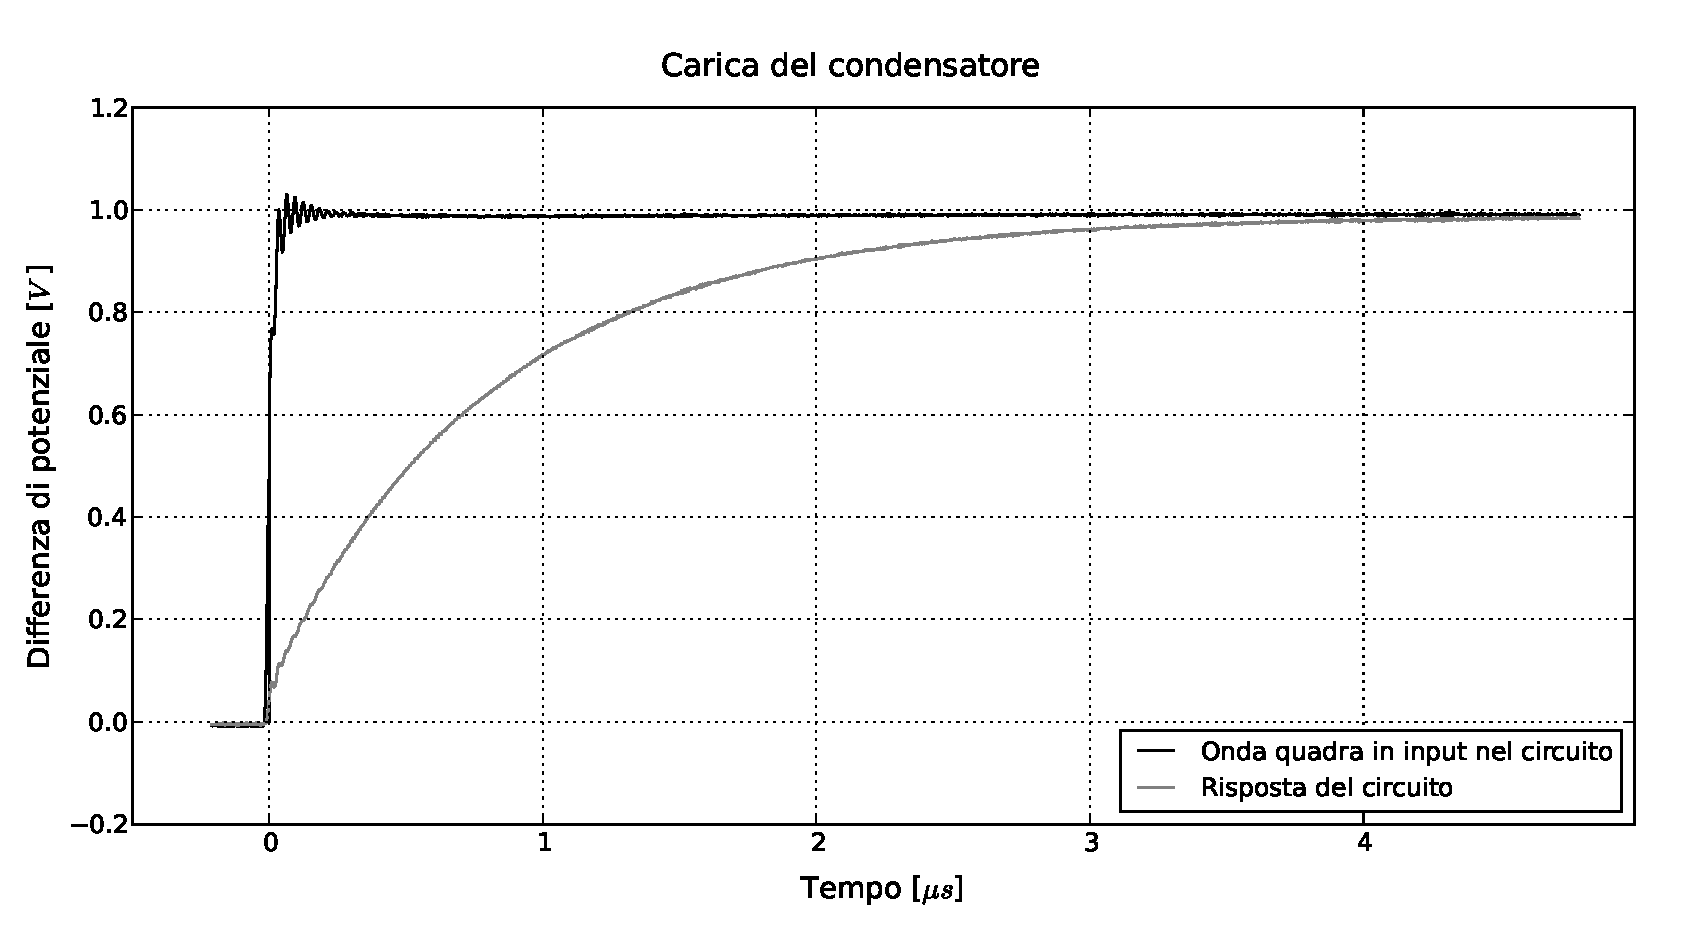
\includegraphics[width=\textwidth]{figure3.eps}%{Res_70.eps}
        \caption{***}
        \label{fig:1}
\end{figure}